\chapter{Les attracteurs de Lorenz}
Tout d’abord commençons par définir rapidement et sans rentré dans les détails mathématiques ce qu’est un attracteur,
 il s’agit d’un ensemble ou d’un espace vers lequel un système dynamique évolue de manière
 irréversible en l’absence de perturbation, le concept d’attracteur est l’une des bases de la théorie du chaos. 
 Dans cette partie nous allons nous concentrer sur l’attracteur de Lorenz, il s’agit d’un attracteur
représentant l’évolution du système dynamique différentiel de Lorenz. Cet attracteur est caractérisé d'attracteur étrange, cela signifie qu'il n'est pas continue, mais formé point par point par la dynamique du système.\\

Le système de Lorenz s'écrit: 
\[
    \left\{
    \begin{array}{rcl}
        \dfrac{dx}{dt}&=&\sigma[y-x]\\
        \dfrac{dy}{dt}&=&x(\rho-z)-y\\
        \dfrac{dz}{dt}&=&xy-\beta z\\
    \end{array}
    \right.
\]
Ces équations sont un modèle très simplifier crée par Lorenz pour modélisé le fonctionnement 
de l’atmosphère terrestre. Il a décidé de cherché un modèle simple car 
les équations décrivant l’atmosphère de façon précise était beaucoup trop compliqué à résoudre
 numériquement à l’époque de Lorenz et il souhaitais pouvoir étudié  le phénomène de convection
de Rayleigh-Bénard à l’aide de son modèle simplifié.\\


Dans ces équations: \\
$\sigma$  correspond au nombre de Prandtl, il s'agit d'un nombre sans dimension obtenu en calculant le rapport entre la diffusivité de la quantité de mouvement et ça diffusivité thermique.\\\\
$\rho$    correspond au nombre de Rayleigh, il s'agit d'une valeur utilisé en mécanique des fluides, il permet de caractérisé le transfert de chaleur au sein d'un fluide \\\\
$\beta $  est une valeur dépendand de la couche de l'atmosphère\\\\
$x$, $y$, $z$ représente l'état du système au court du temps, remis dans leur context physique, $x$ est proportionnel à l'intensité du mouvement de convection, $y$ est proportionnel à la différence de température entre les courants ascendants et descendants. $z$ est proportionnel à l'écart du profil de température vertical par rapport à un profil linéaire.    

\section{Dimension mathématique}

\subsection{Equilibres du modèle}
Nous allons nous intéresser aux point auxquelles le modèle est stable, c’est-à-dire les points d’équilibre $(x,y,z)$ vérifiant $x'=y'=z'=0$, cela revient a résoudre le syteme suivant :\\
\[
    \left\{
    \begin{array}{rcl}
        \sigma(y-x)&=&0\\
        x(\rho-z)-y&=&0\\
        xy-\beta z&=&0\\
    \end{array}
    \right.
\]\\

Avec $\sigma$, $\rho$ et $\beta$ des réels positif.

On remarque que $x=y=z=0$ est une solution évidente de ce système quelque soit les valeurs de $\sigma$, $\rho$ et $\beta$.
A l'aide d'un logiciel de calcule formel, on résoud ce système et l'on trouve des solutions dépendand de $\sigma$, $\rho$, $\beta$ et particulièrement de la valeur de $\rho$, en effet on trouve:\\

Si $\beta(\rho-1)\geq 0$ alors $x= \pm \sqrt{(\beta(\rho-1)}$, $y= \pm \sqrt{(\beta(\rho-1)}$ et $z=\rho-1$\\
autrement dit lorsque $\rho\geq 1$ le système admet 3 points d'équilibre à savoir:\\
 $(\sqrt{(\beta(\rho-1)}; \sqrt{(\beta(\rho-1)}; \rho-1)$, $(-\sqrt{(\beta(\rho-1)}; -\sqrt{(\beta(\rho-1)}; \rho-1)$ et $(0,0,0)$\\\\
 dans le cas ou $\rho < 1$ il admet un seul point d'équilibre à savoir $(0,0,0)$\\
 
\subsection{Stabilité des points d'équilibre}
Les point d'équilibre trouvé précédement ne sont pas toujours stable, l'équilibre peut être stable ou instable, les conditions de stabilité de ses points est déterminée par l'étude du signe de la partie réel des valeurs propres de la matrice jacobienne $A$ obtenue linéarisant le système autour d'un point d'équilibre, cette partie étant trop technique pour nous, on se permet d'admètre l'expression de la matrice jacobienne $A$ et l'on se contentera d'expliqué globalement la méthode utilisé sans rentré dans les détails, car la méthode utilisé fait appel à des notions d'étude de stabilité des équilibres que nous n'avons pas. On admet donc également que si le signe de toutes les valeurs propres est négatif, alors l'équilibre est stable et instable sinon \\\\ 
$A$ a pour expression :\\\\
$$A=
\begin{pmatrix}
    -\sigma & \sigma & 0\\
    \rho & -1 & -x\\
       y & x & -\beta 
\end{pmatrix}\\\\
$$
Interessons nous à la stabilité du point d'équilibre $(0,0,0)$, on a alors:\\\\
$$A=
\begin{pmatrix}
    -\sigma & \sigma & 0\\
    \rho & -1 & 0\\
       0 & 0 & -\beta 
\end{pmatrix}\\\\
$$
les valeurs propres de A sont alors les solutions de
 $det(A-\lambda)=(\sigma*\rho-(\lambda+1)*(\lambda+\sigma))*(\lambda+\beta) $

 En resolvant, on trouve alors trois solution: $\lambda_{1}=\dfrac{\sqrt{4*\sigma*\rho+\sigma^2-2*\sigma+1}-\sigma-1}{2}$, $\lambda_{2}=\dfrac{-(\sqrt{4*\sigma*\rho+\sigma^2-2*\sigma+1}+\sigma+1)}{2}$, $\lambda_{3}=-\beta$\\\\

 On constate que le signe de  $\lambda_{1}$ et $\lambda_{2}$ dépend de $\rho$, en effet si $\rho<1$ alors $\lambda_{1}$ est négative tout comme $\lambda_{2}$ et $\lambda_{3}$, dans ce cas l'équilibre du point d'équilibre $(0,0,0)$ est stable. Cependant, si $\rho>1$, alors $\lambda_{1}$ est positive, donc l'équilibre n'est pas stable.\\\\
 En procédant de façon similaire on peut déterminer la valeur critique de $\rho$ pour laquelle l'équilibre des deux autres points est instable. Ainsi si $\rho > \dfrac{\sigma(\sigma+\beta+3)}{\sigma-\beta-1}$ l'enssemble des points d'équilibres est instable et le système adapte un comportement particulié.
 \section{Visualisation graphique}
Après avoir apréhendé l'attracteur de Lorenz sous sa forme mathématiques, nous allons nous intéresser a ça représentation graphique que les parties précedentes vont nous aider à comprendre. Pour représenté l'attracteur de Lorenz, nous avons écrit un algorithm python qui résoud le système différentiel de Lorenz en fonction du temps et de conditions initiales (à l'aide d'un solveur deja existant) et nous avons affiché la courbe correspondante.\\

\begin{figure}
        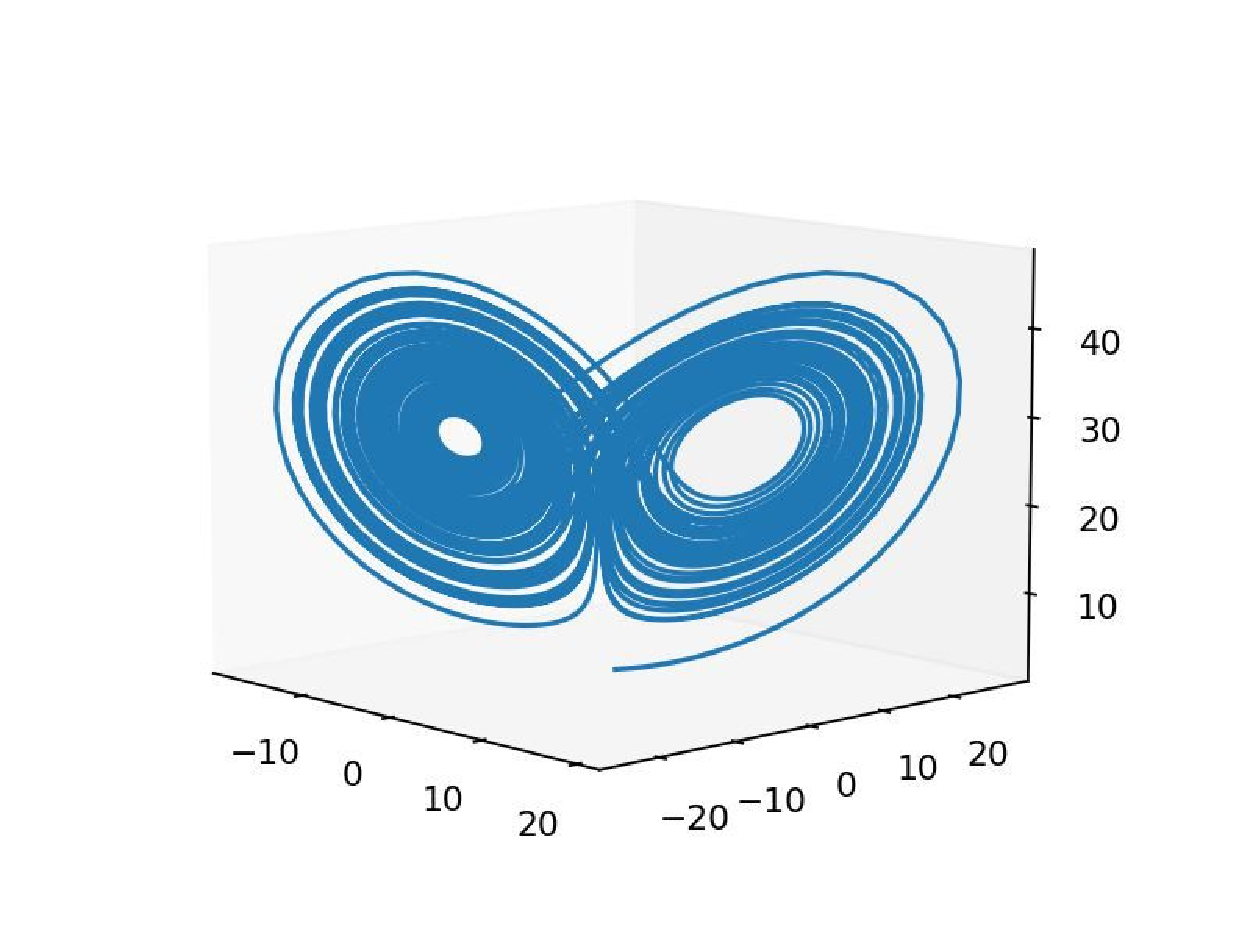
\includegraphics[width=\textwidth]{Attracteur1.pdf}
        \caption{Attracteur de Lorenz pour $\rho=28$, $\sigma=10$ et $\beta=\dfrac{8}{3}$} 
\end{figure} 

On obtient un graphique en trois dimension a l'allure étrange, les valeurs de $\rho$, $\sigma$ et $\beta$ sont les valeurs classique utilisé pour représenter ce système car ce sont les valeurs historique utilisé par Lorenz et car elle permette d'exhibé sont comportement chaotique. Les valeurs des conditions initiales sont pour ce graphique $(1,1,1)$. Ce qu'on observe est en effet un attracteur, car quelque soit les conditions initiales, la trajectoire se retrouvera a évolué dans la zone de l'attracteur.\\\\
Essayons maintenant de comprendre pourquoi obtient on ce graphique. L'aspect de l'attracteur de Lorenz est en grande partie du à la stabilité ou l'instabilité des point d'équilibre dont nous avons parlé précédement, représentons l'attracteur pour $\rho=\dfrac{1}{2}$, $\sigma=10$ et $\beta=\dfrac{8}{3}$  

\begin{figure}
    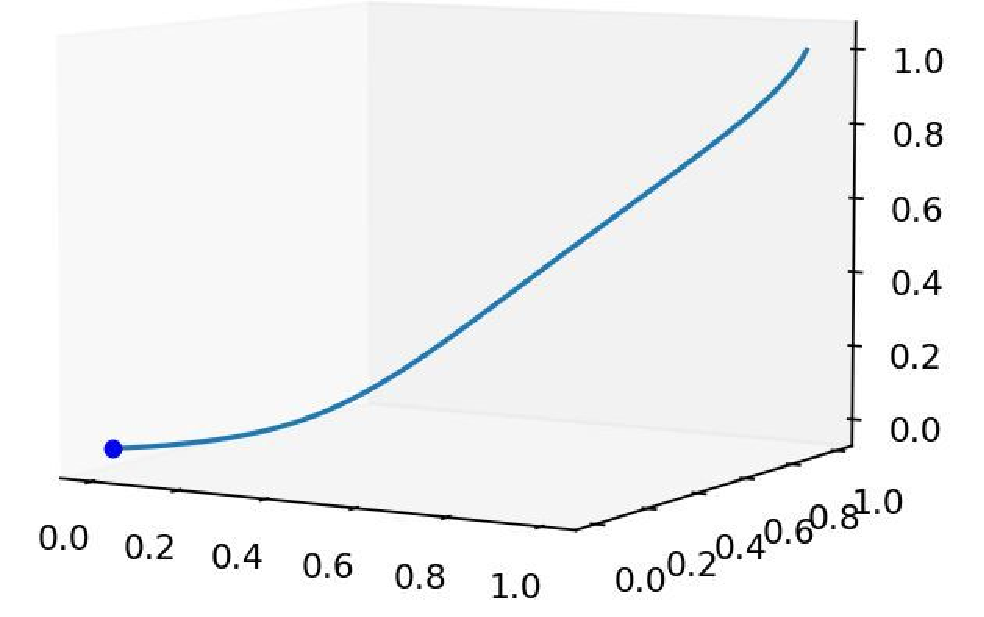
\includegraphics[width=\textwidth]{rho_stable.pdf}
    \caption{Attracteur de Lorenz pour $\rho=\dfrac{1}{2}$, $\sigma=10$ et $\beta=\dfrac{8}{3}$} 
\end{figure}
On constate que le système évolue vers le seul point d'équilibre stable $(0,0,0)$ car $\rho<1$

représentons maintenant l'attracteur pour $\rho=10$, $\sigma=10$ et $\beta=\dfrac{8}{3}$

\begin{figure}
    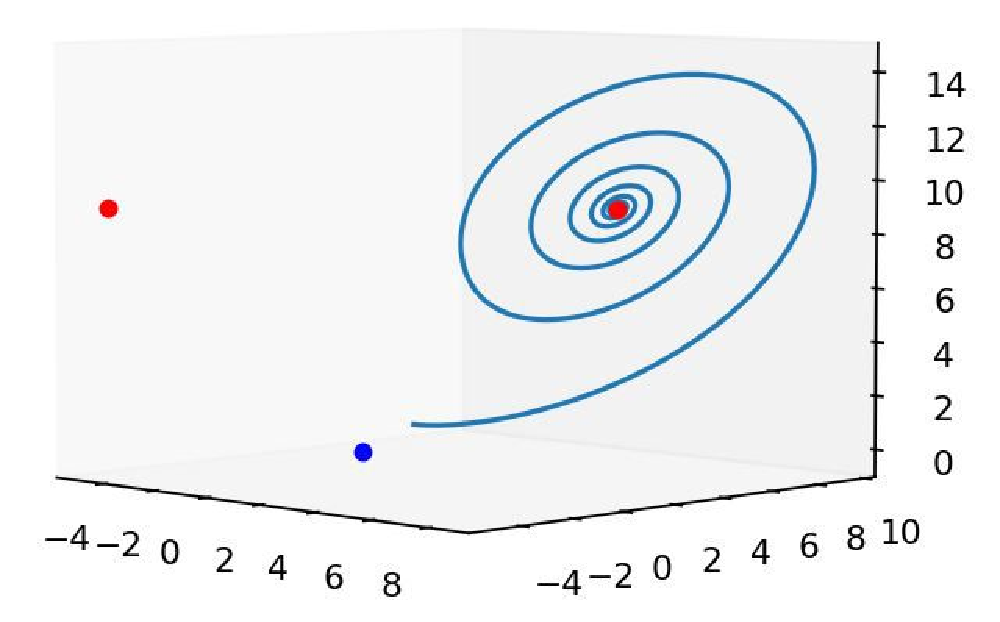
\includegraphics[width=\textwidth]{rho_stable1.pdf}
    \caption{Attracteur de Lorenz pour $\rho=10$, $\sigma=10$ et $\beta=\dfrac{8}{3}$} 
\end{figure}

On observe ici que le système évolue vers l'un des deux point d'équilibres représenté par des point rouge sur le graphique, cela s'explique car dans ce cas $\rho>1$ donc le point $(0,0,0)$ représenté par le point bleu est instable, de plus $\rho < \dfrac{\sigma(\sigma+\beta+3)}{\sigma-\beta-1}=24.74$ donc les deux autres point d'équilibre sont stable, le système évolue donc vers l'un ou l'autre dépendant de la valeurs de $\rho$ et des conditions initiales.  

Enfin représentons l'attracteur pour $\rho=25$, $\sigma=10$ et $\beta=\dfrac{8}{3}$

\begin{figure}
    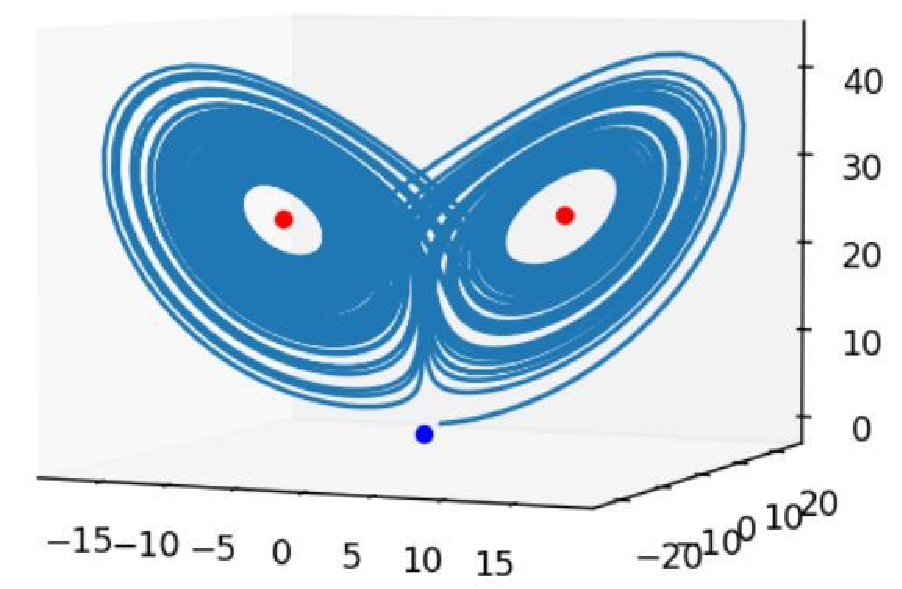
\includegraphics[width=\textwidth]{rho_instable.pdf}
    \caption{Attracteur de Lorenz pour $\rho=25$, $\sigma=10$ et $\beta=\dfrac{8}{3}$} 
\end{figure}

Il n'est pas simple de comprendre ce qu'il ce passe sur ce graphique, la valeur critique de $\rho=24.74$ a été dépassé, alors il n'y a plus de point d'équilibre stable. Le système orbite donc autour de ses point d'équilibre instable passant de l'un à l'autre de façon imprédictible.

A l'aide d'un graphique on peut également observer la forte dépendace aux conditions initiales qui caractérise les systèmes chaotiques. En traçant deux attracteur avec une couleur différente sur le même graphique et en changeant très légèrement l'une des trois conditions initiale, on observe que les deux attracteur ne se superposent pas.

\section{Dimension expérimentale}